\chapter{Разработка методик наполнения и анализа образовательных данных в системе электронного обучения} \label{chapt3}


\section{Метод интеграции учебных материалов из сторонних источников семантических данных} 
\label{sect3_1}

Технологии Semantic Web и Linked Data позволяют использовать онтологии для хранения, сбора и распространения данных. Одним из преимуществ данных технологий является повторное использование данных. В Интернете существует множество открытых источников с данными, при описании которых были использованы онтологии верхнего уровня. Данные источники могут быть использованы для наполнения системы электронного обучения. Автоматизация и разработка методов наполнения онтологий является одной из главных задач в реализации механизмов поддержки учебных материалов в актуальном состоянии в системе электронного обучения.

В разработанном методе для сбора данных в формате RDF в системе электронного обучения используются провайдеры данных. Провайдеры данных - это программные автономные модули, поддерживающие  автоматическое обновление связных данных хранилища системы из сторонних источников. Провайдеры позволяют преобразовывать структурированные данных различных форматов в формат RDF. Каждый провайдер обладает своим контекстом для дальнейшего управления собранными данными. Система электронного обучения использует связанные данные из хранилища для предоставления пользователям учебных материалов.

С помощью провайдеров данных система электронного обучения  наполняет онтологии учебных материалов и тестов. Система производит сбор данных из электронных библиотек. Одним из примеров использования разработанного метода является сбор данных системой электронного обучения из библиотеки The British National Bibliography(BNB). BNB предоставляет открытый доступ к библиографической информации в формате RDF. Библиографические данные описываются с помощью онтологии верхнего уровня BIBO и прочих опубликованных в сети прикладных онтологий. Система электронного обучения собирает информацию о книгах и публикациях из BNB и предоставляет возможность преподавателям и авторам  связывать электронные курсы с объектами BNB, используя свойство <<hasResource>> онтологии учебных материалов.

С помощью разработанного метода система электронного обучения позволяет задавать определения для концептов предметных областей. Одним из способов автоматизации наполнения онтологии концептов и предметных областей является использование внешней базы знаний или таксономии. В качестве такой базы знаний в системе электронного обучения может быть использована база знаний DBpedia. DBpedia предоставляет точку доступа SPARQL для получения информации, которая была извлечена из Wikipedia. Провайдер данных автоматически создает определения, для концептов предметной области используя запросы к точке доступа SPARQL. Для минимизации неоднозначности значения концептов при произведении запросов провайдером к точке доступа SPARQL в запросах используется дополнительная фильтрация по категориям относящимся к предметной области концепта. 

Разработанный метод поддерживает ручное связывание концепта предметной области в системе электронного обучения с объектом базы знаний. Для этого у выбранного концепта создается свойство <<owl:saneAs>> с URI объекта внешней базы знаний. В дальнейшем провайдер автоматически подгружает актуальную информацию о концепте предметной области из внешних источников.



\section{Метод преобразования структурированных учебных материалов в семантический формат} \label{sect3_2}

Множество источников в Интернете хранят структурированные данные не в формате RDF. Тесты и учебные материалы университета могут храниться в формате XML, а электронная библиотека предоставлять информацию о публикациях через REST API. Разработанный метод агрегации данных в структурированных форматах предлагает использовать алгоритмы конвертации данных в провайдерах для интеграции структурированных данных в онтологии системы.

Портал учебных изданий Университета ИТМО предоставляет доступ к информации, о публикациях используя точку доступа REST API. Разработанный метод использует предопределенные разработчиком Groovy скрипты при обработке данных в провайдере для преобразования данных из REST API в RDF триплеты. В ходе преобразования могут быть использованы внешние и внутренние словари и онтологии для аннотирования полученных данных. В примере с учебными изданиями может быть использовано аннотирование данных с помощью онтологии BIBO для сохранения информации о публикациях и книгах. 

Другим распространенным методом хранения и передачи учебных материалов в электронных курсах является передача данных в формате XML. Для преобразования учебных материалов из XML формата в формат RDF необходимо описать отображение данных. Отображение описывается в формате XML в виде специальных правил задающих соотношение между данными в элементах и атрибутах XML и онтологическими индивидами и свойствами. Описанное отображение передается в провайдер, разработанный для обработки XML данных. Далее провайдер на основе описанного отображения и указанных внешних источников производит сбор и конвертацию в семантических формат учебных материалов в формате XML. Провайдер использует функции XPath для извлечения информации об объектах и их свойствах из XML данных. Извлеченная информация преобразовывается в RDF/XML формат и аннотируется с помощью установленных онтологий на основе описанного отображения. Агрегация данных производится в автоматическом режиме с заданной периодичностью, что позволяет автоматически актуализировать учебные материалы.

Одним из примеров применения данного метода является агрегация тестов электронных курсов из открытого хранилища учебных материалов ИТМО. Скрипт производит сбор и формирование XML файлов с тестами из открытого хранилища. Далее провайдер на основе описанного отображения преобразовывает и сохраняет данные в семантическое хранилище. В приложении \ref{APP_B_XML_MAP} описан пример отображения и результаты работы провайдера при преобразовании тестов в формате XML в семантических формат.

Таким образом, система электронного обучения с использованием семантических технологий может агрегировать и интегрировать книги, публикации, тесты и прочие учебные материалы, опубликованные в структурированном формате на внешних источниках. Интеграция учебных материалов в систему электронного обучения, основанную на семантических технологиях, позволяет преподавателям и авторам использовать в своих электронных курсах готовые учебные материалы из сторонних источников.  



\section{Использование алгоритмов обработки естественного языка для создания связей в онтологиях} \label{sect3_3}

Для наполнения онтологий системы можно использовать не только данные внешних источников, но и данные самой системы. Данные хранящиеся в онтологии системы и связанные семантическими связями позволяют создавать новые связи на основе предопределенных правил. Одним из методов связывания данных онтологии является применение алгоритмов обработки естественного языка NLP (Natural Language Processing). Используя данный подход можно извлекать семантические связи из текстовой информации объекта онтологии. Разработанный метод позволяет системам электронного обучения на основе семантических технологий, использовать NLP алгоритмы для поиска концепты предметных областей в текстах заданий тестов.

Учитывая небольшой размер образца и предустановленный набор концептов, шаблоны POS-tag в совместном использовании с синтаксическими шаблонами являются наиболее предпочтительным методом извлечения концептов предметных областей из заданий тестов \cite{hulth2003improved} \cite{khokhlova2012lexico} \cite{bolsh2007lexico}. Около десяти типичных составных шаблонов концептов было использовано для извлечения концептов-кандидатов.  После извлечения концепты-кандидаты приводились к канонической форме с использованием предустановленных словарей.

Для извлечения концептов предметных областей была использована лингвистическая платформа NooJ \cite{silberztein2002nooj}. NooJ обладает мощным механизмом регулярных выражений поиска, позволяющим комбинировать различные POS-tag шаблоны в единую грамматику для запроса к тексту. Для обработки русскоязычного текста был разработан набор грамматик и словарей. Данные словари и грамматики полностью покрывают словарь заданий теста. Для генерации словарей и грамматик для англоязычных ресурсов были использованы стандартные средства NooJ. Несколько деривационных парадигм было описано с помощью преобразователей NooJ и связано с лексическими сущностями. Применение деривационных парадигм позволяет генерировать основные леммы для лексических сущностей. Алгоритм извлечения концептов предметных областей из текста с использованием платформы NooJ состоит из следующих шагов:

\begin{itemize}
\item тест задания подгружается в платформу NooJ, что приводит к его лингвистическому анализу, используя разработанные словари;
\item в результате анализа платформа NooJ формирует текст с аннотациями, содержащими морфологическую и семантическую информацию о каждом слове;
\item применяя запросы на основе POS-tag шаблонов, платформа NooJ формирует список концептов-кандидатов.
\end{itemize}

Для применения алгоритма в других предметных областях и на других языках необходимо сформировать соответствующие словари, грамматики и шаблоны извлечения концептов предметных областей.

Для связывания концептов-кандидатов с концептов предметных областей системы с помощью лемм, концепты системы должны пройти лемматизацию. Каждый концепт системы обладает свойством-значением <<lemma>>. Концепт предметной области в  системе хранит в данном свойстве все свои леммы.

Для реализации алгоритма связывания заданий тестов и концептов предметных областей был разработан провайдер данных. Провайдер принимает на вход ссылку на объект курса и производит создание ссылок между заданиями и концептами. Общий алгоритм работы провайдера данных представлен на рисунке \ref{img:nlp_main_alg}.

\begin{figure} [h] 
  \center
  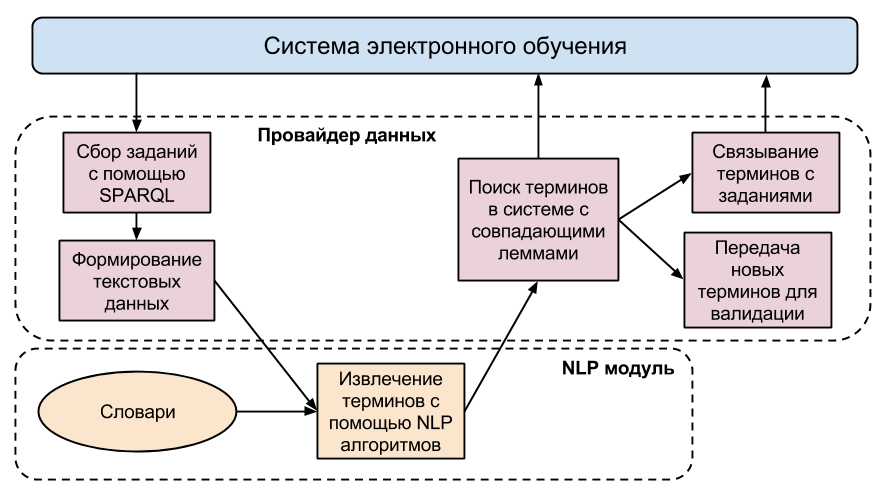
\includegraphics [width=0.95\textwidth] {nlp_main_alg}
\caption{Алгоритм работы провайдера извлечения концептов с использованием NLP алгоритмов.}
  \label{img:nlp_main_alg}  
\end{figure}

Алгоритм состоит из следующих шагов:

\begin{itemize}
\item провайдер собирает список заданий курса, используя запросы SPARQL;
\item происходит формирование текстовых данных для каждого задания, используя информацию о вопросах и ответах;
\item провайдер данных запускает NLP алгоритмы в платформе NooJ для текстовых данных каждого задания;
\item провайдер формирует список концептов-кандидатов содержащих каноническую форму и набор лемм;
\item производится поиск концептов предметной области в системе с совпадающими наборами лемм для дальнейшего связывания с концептами-кандидатами;
\item провайдер создает связи между найденными концептами  предметной области системы и заданиями концептов-кандидатов с помощью объектного свойства <<hasTerm>>.
\end{itemize}

Концепты-кандидаты, для которых не были найдены соответствующие концепты предметной области системы, могут быть записаны в онтологию, как новые концепты предметной области системы. Перед записью в онтологию провайдер производит проверку концепта-кандидата на соответствие концепту предметной области. Для проверки используются запросы к базе знаний DBpedia. В случае совпадения названия концепта-кандидата со свойствами <<rdfs:label>> или <<dbpedia-owl:wikiPageRedirects>> объекта из Dbpedia, в онтологии системы создается новый концепт предметной области на основе концепта-кандидата и производится связывание с заданиями теста. При отсутствии совпадений концепт-кандидат помечается провайдером данных как ложный концепт. При SPARQL запросах к базе знаний DBpedia используется фильтрация по предметным областям и категориям с помощью свойства <<dcterms:subject>>.

Данная фильтрация позволяет избежать ошибочных совпадений концептов-кандидатов с концептами из сторонних предметных областей. Проверка считается успешной в случае одного или более найденных совпадений для концепта-кандидата. Для включения нового концепта в систему необходима верификация преподавателя или администратора системы. Алгоритм проверки концептов-кандидатов представлен на рисунке \ref{img:nlp_check_alg}.

\begin{figure} [h] 
  \center
  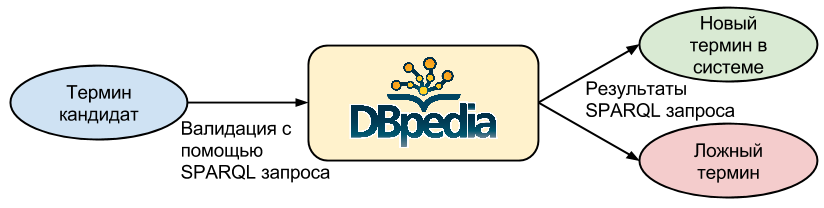
\includegraphics [width=0.95\textwidth] {nlp_check_alg}
\caption{Алгоритм проверки новых концептов-кандидатов.}
  \label{img:nlp_check_alg}  
\end{figure}



\section{Метод анализа качества учебных материалов основе свойств и связей в онтологиях и действий пользователей системы} \label{sect3_4}

Анализ качества учебных материалов производится внутри аналитических модулей системы. Каждый модуль состоит из отдельной аналитической страницы с графиками, таблицами и другими визуальными компонентами. Аналитические страницы основаны на синтаксисе Semantic MediaWiki \cite{krotzsch2006semantic} и хранятся в платформе Information Workbench. Данные графиков, таблиц и визуальных элементов собираются аналитическим модулем с помощью SPARQL запросов к точке доступа.

Связи между концептами, предметными областями и учебными материалами позволяют анализировать содержание электронного курса. Одним из примеров такого анализа является анализ доли использования различных предметных областей в теоретическом материале электронного курса. Анализ строится на основе оценки связей между концептами и лекциями курса. Концепты связаны с определенными предметными областями, что позволяет аналитическому модулю рассчитать с помощью SPARQL-запросов долю использования предметной области в электронном курсе. Предметная область, концепты которой, обладают большим количеством ссылок с лекциями курса, обладает большей долей использования в электронном курсе. Интерфейс анализа использования предметных областей в электронном курсе представлен в приложении \ref{APP_C_COURSE_FIELD}. 

Одним из примеров метода анализа качества учебных материалов является анализ покрытия лекций курса тестами и заданиями. В онтологии системы лекции и тесты связаны с определенным модулем курса. В результате работы алгоритмов по наполнению онтологий лекции и задания тестов могут быть связаны с определенными концептами предметной области. Таким образов происходит косвенное связывание лекций и тестов через концепты предметной области. Система может предоставить статистику по количеству концептов предметной области лекций модуля использованных в тестах модуля. Если концепт лекции использован в задании теста, он считается покрытым в данном модуле. Каждый модуль имеет аналитическую страницу. 

Аналитическая страница модуля содержит следующую статистическую информацию:

\begin{itemize}
\item количество покрытых и непокрытых концептов предметной области в модуле,
\item общий процент покрытия модуля тестами на основе отношения покрытых концептов к общему количеству концептов,
\item облако тегов концептов предметной области модуля демонстрирующее качество и степень покрытия каждого концепта,
\item список непокрытых концептов модуля, которые были использованы в лекциях, но не были использованы в заданиях тестов.   
\end{itemize}

Интерфейс аналитической страницы модуля позволяет получать информацию о покрытии тестами каждой лекции в отдельности. Интерфейс представлен в приложении \ref{APP_C_COVER}.

Другим подходом к анализу учебных материалов является выявление проблемных  концептов предметной области в модуле курса. Проблемными концептами предметной области являются концепты, при изучении которых у студентов возникают наибольшие затруднения. Статистика по результатам прохождения студентами тестов, правильные и неправильные ответы на задания связанные с определенными концептами предметной области позволяют рассчитать рейтинг знания каждым студентом определенного концепта. Используя данный рейтинг, преподаватель, может получить список концептов предметной области курса, которых студенты знают хуже всего. Это позволит преподавателю вносить коррективы в учебные материалы и учебный процесс. В текущей реализации данного аналитического модуля рейтинг проблемного концепта рассчитывается делением количества неправильных ответов на количество правильных ответов на задания связанные с данным концептом. В будущем данная формула будет усложнена с учетом сложности заданий и глобального рейтинга концептов студентов. Рейтинг проблемных концептов для модуля составляется с помощью следующего  SPARQL-запроса:

\begin{verbatim}
    SELECT ?term 
        (count(?correct_answer) AS ?correct_answer_count)
        (count(?answer) AS ?answer_count)
        ((2*?correct_answer_count - ?answer_count) 
            AS ?rank) 
    WHERE{
        ?module learningRu:hasTest ?test  . 
        ?test ifmotest:hasGroupOfTasks 
            ?group_of_tasks .        
        ?group_of_tasks ifmotest:hasTask ?task .      
        ?test_element lres:hasTask ?task .
        ?test_element lres:hasAnswer ?answer .
        ?task learningRu:hasTerm ?term .       
        OPTIONAL { 
            ?task ifmotest:hasCorrectAnswer 
                ?correct_answer
            filter( ?correct_answer = ?answer)
        }         
    }
    GROUP BY ?term 
    ORDER BY ASC(?rank)
\end{verbatim}

Анализ проблемных концептов предметной области реализован на аналитической странице модуля. Аналитическая страница модуля включает в себя список проблемных концептов с рейтингами и диаграмму отношений между пятью самыми проблемными концептами модуля. Интерфейс аналитики проблемных концептов представлен в приложении  \ref{APP_C_PROBLEM}.

Аналитика учебного материала, основанная на использовании семантических связей между объектами системы, позволяет строить различные запросы для оценки качества учебных материалов. Полученная информация позволяет преподавателям и авторам курса выявлять и исправлять устаревшие, ошибочные и неточные учебные материалы, основываясь на динамике образовательного процесса и его структуре.



\section{Автоматизированная оценка знаний студентов на основе анализа онтологий} \label{sect3_5}

Подход к автоматизированному анализу знаний и рейтингов студентов системы электронного обучения основан на семантическом анализе действий студентов в системе электронного обучения в проекции образовательного процесса и учебных материалов. Целью подхода является автоматизированный вывод рейтинга знаний студента по определенной предметной области учебной дисциплины. Рейтинг знания предметной области зависит от рейтингов входящих в нее концептов. Расчет рейтинга знания концепта зависит от показателей оценки действий студента в системе. Набор показателей может варьироваться в зависимости от возможных действий студентов в системе, структуры онтологии и необходимой точности вычислений. В предложенном алгоритме  используются показатели: 

\begin{itemize}
\item первое знакомство студента с концептом на основе первого чтения лекции,
\item ответы студента на тесты связанные с концептом. 
\end{itemize}

Расчет рейтинга знаний предметной области для студента  производится с учетом значимости(важности) концептов предметных областей в образовательном процессе.

Рейтинг знания концепта, как и рейтинг знания предметной области, варьируется от 0 до 1. Показатель знакомства с концептом является бинарным показателем и обозначает факт изучения студентом концепта предметной области с использованием теоретического материала. В разработанном подходе изучением концепта является завершение студентом лекции связанной с данным концептом в системе электронного обучения. Изучить концепт предметной области студент может только один раз. В разработанном подходе данный показатель составляет 15\% от общего рейтинга знаний концепта.

Показатель проверки знания концепта предметной области с помощью тестов основан на статистическом анализе правильных и неправильных ответов студента на задания учебных курсов, которые связаны с данным концептом. В разработанном алгоритме данный показатель составляет 85\% от общего рейтинга знаний концепта. Показатель рассчитывается как нижняя граница доверительного интервала Вильсона для параметра Бернулли по количеству правильных и неправильных ответов, используя формулу:

$$
    R_t = \frac{p+\frac{1}{2n}z_{1-\alpha/2}^2 \pm z_{1-\alpha/2}\sqrt{\frac{p(1-p)}{n}+\frac{z_{1-\alpha/2}^2}{4n^2}}{} }{1+\frac{1}{n}z_{1-\alpha/2}^2},
$$

где \(z_{1-\alpha/2}\) - квантиль от от \(1-\alpha/2\) стандартного нормального распределения, \(p\) - доля правильных ответов, \(n\) - общее количество ответов. 

Сумма двух полученных показателей для концепта предметной области в соответствии с их долями является общим рейтингом знания концепта. Предметные области и концепты в соответствии с разработанной моделью не зависят от учебных материалов и могут повторно использоваться во множестве учебных курсов. Связи между концептами, описывающие необходимость одного концепта для изучения другого, позволяют рассчитать значимость концепта в образовательном процессе. Чем больше концептов, для изучения которых необходим определенный концепт, тем выше значение данного концепта. При расчете учитывается количество концептов на разных уровнях зависимости. Уровнем зависимости является глубина косвенной зависимости одного концепта от другого через набор концептов. Например, на втором уровне зависимости находятся концепты, зависимые от концептов, зависимых от рассматриваемого концепта. Значение концепта рассчитывается с использованием трех уровней зависимости по формуле: 

$$
    W_t = \frac{1}{e}+\sum_{k=1}^{3}\frac{n_{tk}}{e^k}, 
$$

где \(n_{tk}\) - количество концептов, связанных с данным концептом на каждом уровне зависимости, \(k\) - номер зависимого уровня, \( \frac{1}{e} \) - константное значение концепта. 

Вклад в значимость концепта потомком убывает по экспоненте в зависимости от уровня потомка концепта. Данная функция была выбрана для ограничения количества рассматриваемых уровней потомков до трех. На четвертом уровне потомков вклад в значимость концепта незначителен, а значит, может быть опущен. У каждого концепта предметной области есть собственное значение значимости, что позволяет регулировать значимость концептов без потомков. Пример расчета значимости концепта предметной области представлен на рисунке \ref{img:algo_importance_exmpl}.

\begin{figure} [h] 
  \center
  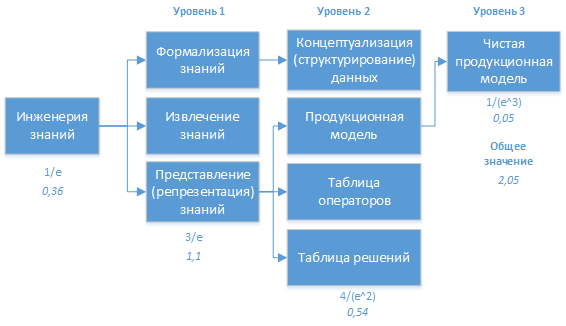
\includegraphics [width=0.95\textwidth] {algo_importance_exmpl}
\caption{Пример расчета значимости концепта предметной области.}
  \label{img:algo_importance_exmpl}  
\end{figure}

Итоговый рейтинг знания студентом предметной области учебной дисциплины рассчитывается как сумма рейтингов концептов, входящих в предметную область. При расчете необходимо учитывать относительную значимость концепта в предметной области. Для этого необходимо рассчитать суммарную значимость предметной области, используя формулу:

$$  
    W_f = \sum_{i=1}^{n}W_{ti},
$$

где \(W_{ti}\) - значимость концепта предметной области, \(n\) - количество концептов в предметной области.

Относительная значимость концепта в предметной области рассчитывается по формуле:

$$
    D_t = \frac{W_t}{W_f},
$$

где \(W_t\) - значимость концепта, \(W_f\) - значимость предметной области.

Рейтинг предметной области является суммой рейтингов концептов данной предметной области в соответствии с их относительными значениями значимости:

$$
    R_f = \sum_{i=1}^{n} R_{ti}D_{ti},
$$
где \(R_{ti}\) - рейтинг концепта, \(D_{ti}\) - относительное значение значимости концепта в предметной области.

Представленный алгоритм позволяет производить автоматизированную оценку знания студентами предметных областей. Поддержка набора показателей позволяет системе варьировать алгоритмы расчета оценки, добавляя, изменяя и удаляя необходимые показатели. Помимо оценки предметных областей данный подход можно применять к любым объектам образовательного процесса, напрямую или косвенно связанным с концептами предметных областей. Разработанный алгоритм позволяет производить оценку учебных курсов и специальностей.

\clearpage
